\section{General Optimization Methods}

    \begin{frame}{General Optimization Methods}
        \centering
        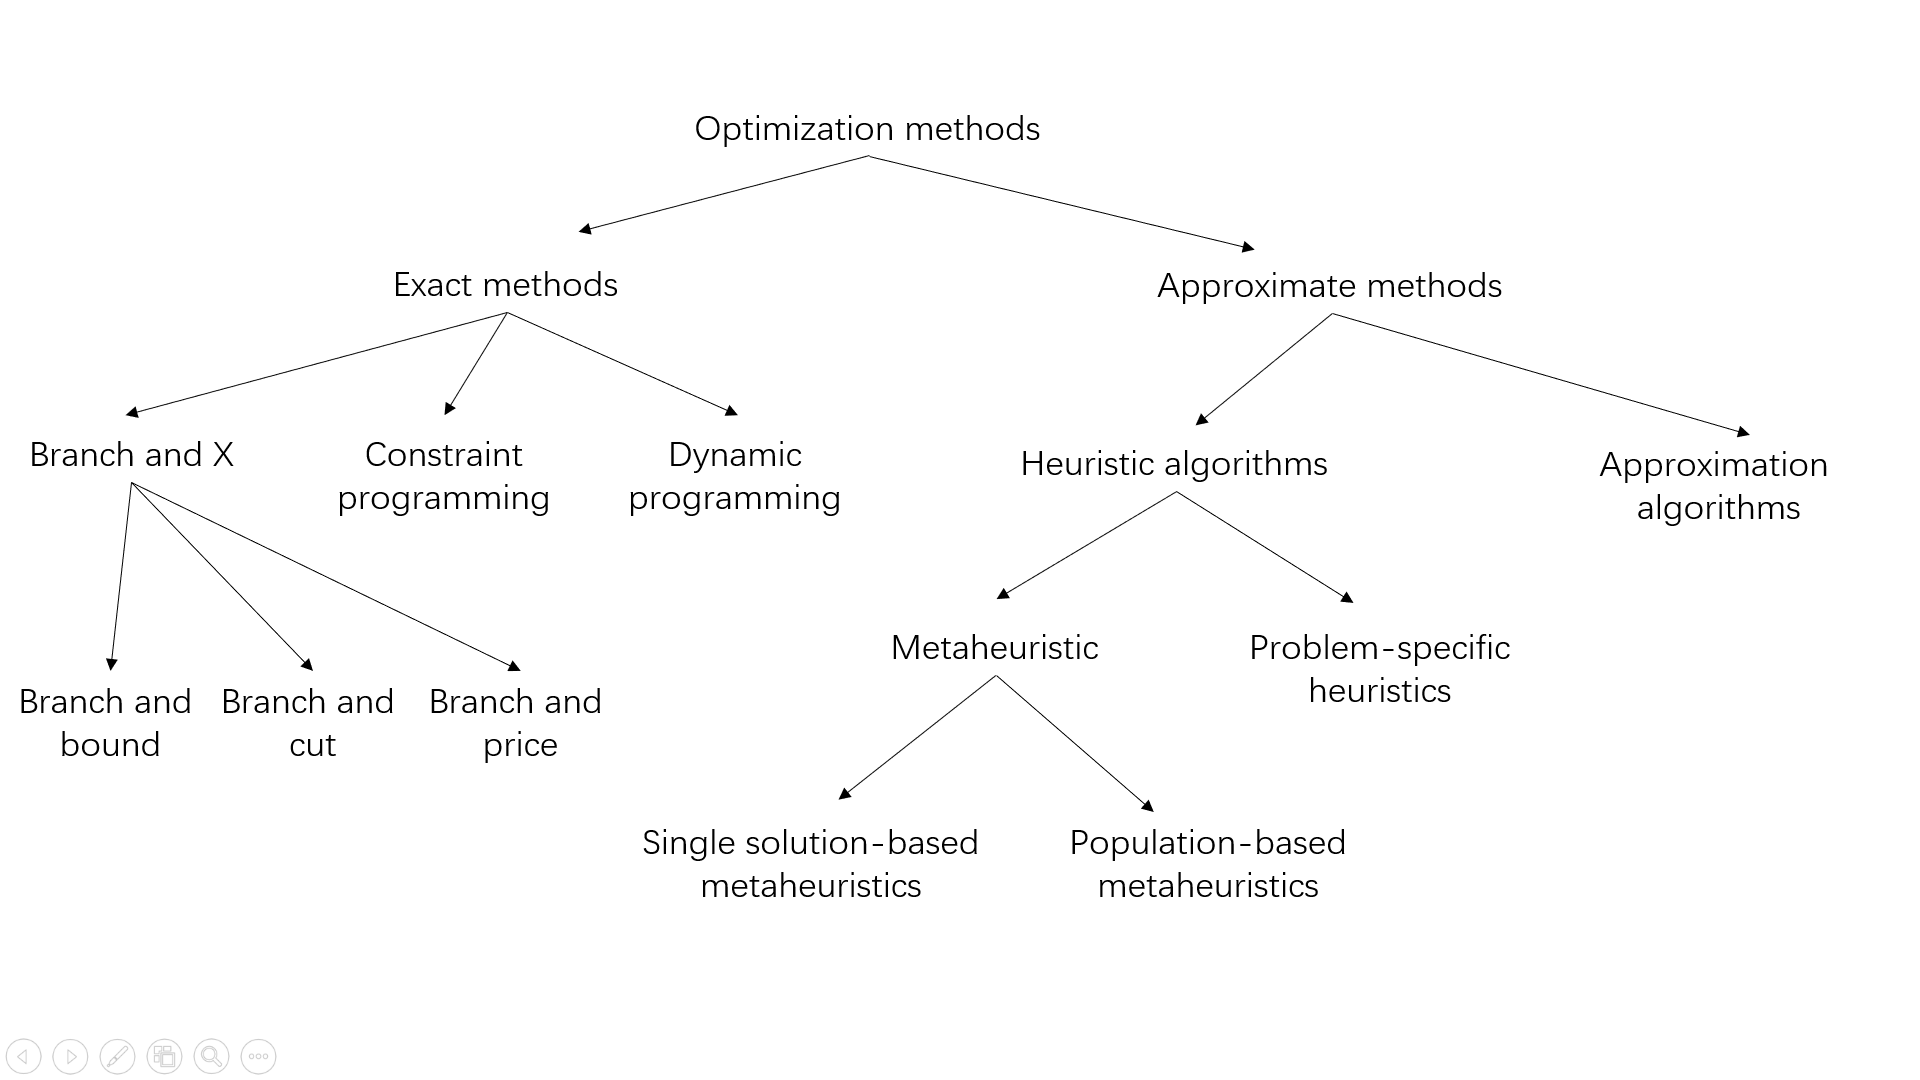
\includegraphics[width = 1\textwidth]{images/opt.png}
    \end{frame}

    \subsection{Exact Methods}
    \frame{\sectionpage}

    \begin{frame}{Exact Methods}
      \begin{itemize}
        \item<+> Branch and X
        \only<2,3,4>{\begin{enumerate}
          \item<+>  Branch and bound
          \item<+>  Branch and cut
          \item<+>  Branch and price
        \end{enumerate}}
      \end{itemize}
      
      \begin{itemize}
        \item Branch and X
        \item<+-> Dynamic programming
        \item<+-> Constraint programming
        \item<+-> Enumeration method
      \end{itemize}
    \end{frame}

    \begin{frame}{Cutting Plane}
      \item facets
    \end{frame}

    \begin{frame}{Branch and price}
      \centering
      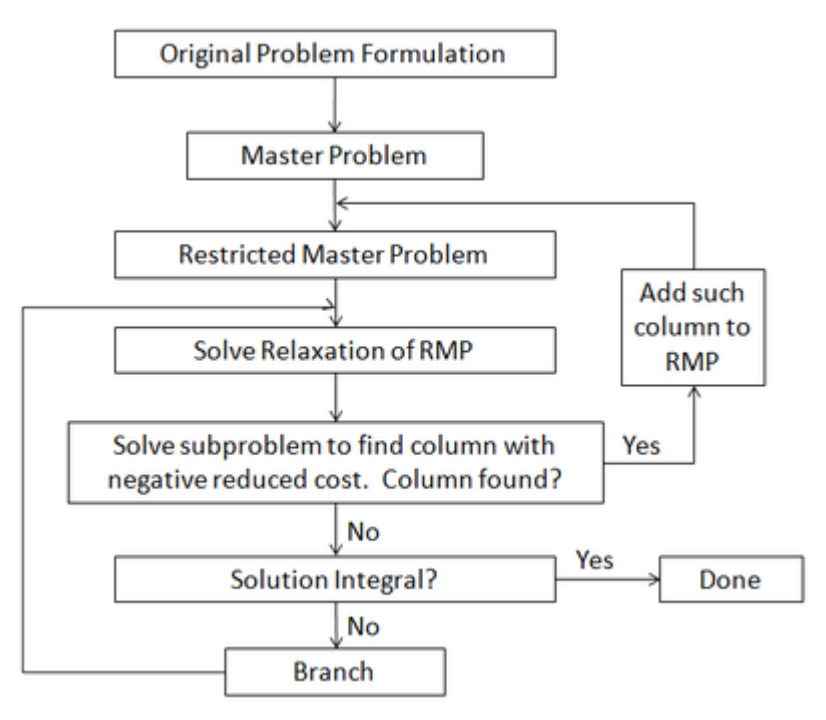
\includegraphics[width = 0.7\textwidth]{images/branch_price.png}
    \end{frame}

    \subsection{Approximate Methods}
    \frame{\sectionpage}

    \begin{frame}{Approximate Methods}
      \begin{itemize}
        \item Heuristic algorithms
        \begin{enumerate}
          \item<+->  Metaheuristic
            \begin{enumerate}
              \item<+>[*] Single solution-based metaheuristics
              \item<+>[*] Population-based metaheuristics
            \end{enumerate}
          \item<+->  Problem-specific heuristics
        \end{enumerate}
        \item<+-> Approximate algorithms
      \end{itemize}
    \end{frame}


    \begin{frame}{Uncertainty Relation}
        \begin{block}{\centering$\sigma_x\sigma_p \geq \frac{\hbar}{2}$}
            The
            \alert{Ramamurti Shankar}
        \end{block}
    \end{frame}
